% Session 04 summaries: designed to be included from an existing main.tex
% No documentclass, packages, or document environment are included.

\section{James D. Fearon -- Rationalist Explanations for War}

\subsection{Central Puzzle and the Bargaining Framework}

The article asks how war can arise between genuinely rational, unitary states whose leaders understand the costs of fighting. Fearon distinguishes this question from explanations based on irrationality or domestic political pathologies. His goal is narrower and foundational.

The key move is to treat war as a bargaining problem. Suppose two states dispute an issue that can be divided along a continuous interval. If state A wins a war with probability p and both states pay positive costs of fighting, then war is a costly lottery. A's expected payoff from war is p minus its costs, while B's is 1-p minus its costs. Because both sides lose something by fighting, there normally exists a set of peaceful divisions that gives each side more than its expected payoff from war. This set is the bargaining range. In the risk-neutral case, the width of the range is essentially the sum of the two sides' costs of war. Risk aversion makes the peaceful range even larger.

This result shifts the explanatory burden. It is not enough to say that a leader expects the benefits of war to exceed the costs. Even if war has positive expected utility, both sides should still prefer a bargain that reproduces the expected distributional outcome without paying the costs of combat. War is ex post inefficient, and this inefficiency normally creates an ex ante space for agreement. A coherent rationalist theory of war must therefore explain why states cannot locate or agree on a settlement inside that range.

\begin{center}
    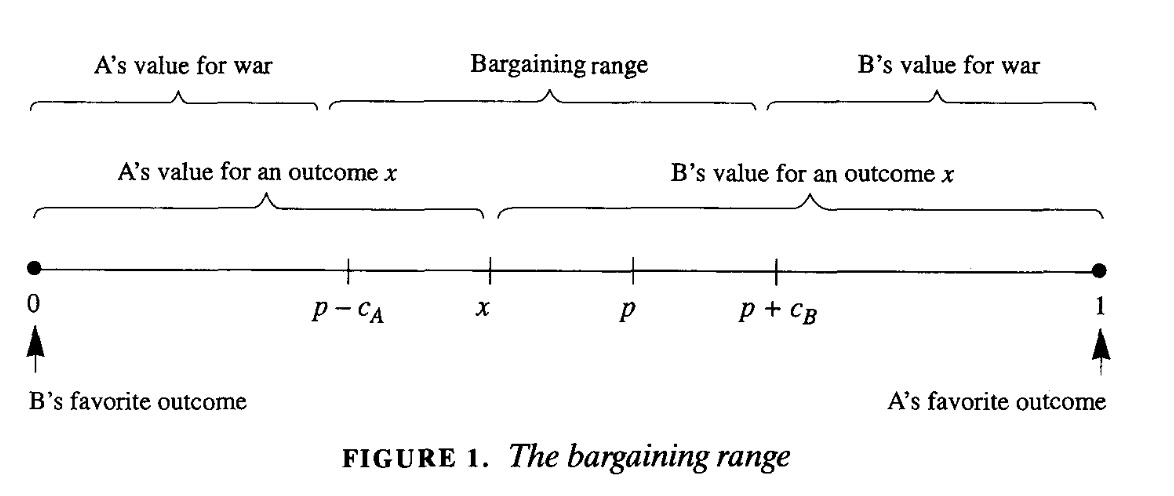
\includegraphics[width=1\textwidth]{images/fearon_rationalist_explanations_war_bargaining_range.jpg}
    \captionof{figure}{\label{fig:fig7_fearon_rationalist_explanations_war_bargaining_range.jpg}%\textit{\parencite[Fig.\(\backsim\)1]{cranmerWhatCanWe2017}}
    }
\end{center}

\subsection{Why Standard Rationalist Arguments Are Incomplete}

Fearon evaluates several familiar explanations.

The central question, then, is what prevents states in a dispute from reaching an ex ante agreement that avoids the costs they know will be paid ex post if they go to war?

\begin{enumerate}
    \item First, \textbf{anarchy} by itself is insufficient. The absence of a world government may permit the use of force, but \textbf{it does not explain why states choose an option that destroys resources when mutually preferable bargains are available}.
    
    \item The \textbf{security dilemma} similarly can generate fear, arms races, and competition, but unless one specifies how the absence of enforceable commitments blocks a peaceful bargain, the argument does not solve the bargaining puzzle.
    
    Security dilemma: the fact that under anarchy one state's efforts to make itself more secure can have the undesired but unavoidable effect of making another state less secure.

    \item Second, the standard \textbf{preventive-war} argument is incomplete. A declining state may fear that a rising state will become stronger and exploit it later. But this immediately raises a bargaining question: why cannot the rising state make concessions today and promise future concessions sufficient to induce the declining state not to attack? The problem is not power shifts in themselves. Preventive war becomes a genuine rationalist explanation \textbf{only when} the changing balance of power creates a \textbf{commitment problem}--when the rising state cannot credibly commit not to use its future strength to revise the agreement.
    \item Third, positive \textbf{expected utility} for war is not enough. Two states can both believe that war is worthwhile relative to the status quo and \textbf{still possess a bargaining range that would make both better off}.
    \item Finally, \textbf{issue indivisibility} is logically capable of eliminating the bargaining range, but Fearon treats it as empirically less compelling. Most international disputes are multidimensional, and side payments, issue linkages, partitions, alternation, or lotteries can often create intermediate outcomes. When issues appear indivisible in practice, the deeper cause may be nationalism, domestic political constraints, or some other mechanism rather than a natural indivisibility of the issue itself.
\end{enumerate}

\subsection{Private Information and Incentives to Misrepresent}
Fearon's first major mechanism combines private information with strategic incentives to misrepresent it. Leaders may possess information about military capabilities, tactics, resolve, or the value they attach to the disputed issue that the opponent does not know. This can create divergent estimates of the likely outcome of war or of the opponent's willingness to fight. Yet simple uncertainty is not sufficient: \textbf{because war is costly, rational states have incentives to reveal information to avoid an inefficient conflict}.

The problem is that bargaining creates incentives to bluff. This logic explains why rational miscalculation can persist.

States can in principle communicate with each other and so avoid a costly miscalculation of relative power or will. The cause of war cannot be simply lack of information, but whatever it is that prevents its disclosure. I argue that the fact that states have incentives to misrepresent their positions is crucial here, explaining on rationalist terms why diplomacy may not allow rational states to clarify disagreements about relative power or to avoid the miscalculation of resolve.

The same reasoning applies to disputes about relative power. Conflicting expectations can shrink or eliminate the apparent bargaining range, but rational actors must have some basis for holding different beliefs. Private information about capabilities is one source. Yet the critical mechanism is again the difficulty of credibly revealing that information. The article therefore recasts many traditional claims about miscalculation as specific bargaining failures produced by asymmetric information and incentives to dissemble.

\section{James D. Fearon -- Rationalist Explanations for War}
\subsection{The central puzzle and Fearon's objective}
Fearon begins from a simple but fundamental puzzle: wars are costly, risky, and destructive, yet they repeatedly occur. Existing explanations can be divided into three broad families. One attributes war to irrationality, psychological biases, or pathologies among leaders. A second focuses on domestic political distortions, in which leaders may enjoy the benefits of war while shifting much of its cost onto soldiers and citizens. Fearon concentrates on a third possibility: whether war can occur even when states are treated as rational, unitary actors whose leaders take the costs and risks of fighting seriously.

This question matters not only for the study of war but also for neorealist international relations theory. If war cannot be explained among rational unitary states, then the roots of conflict must lie primarily in individual or domestic-level defects rather than in the international system itself. Fearon's aim is therefore to identify the set of rationalist explanations that are both logically coherent and empirically plausible.

His central criticism of much of the existing literature is that it asks the wrong question. It is not enough to show that war might have a positive expected value, that states live under anarchy, that one state is declining, or that leaders can miscalculate. Because fighting is costly, rational states should normally have an incentive to search for a negotiated settlement that gives both sides more than they expect to obtain from war after subtracting the costs of fighting. A satisfactory rationalist theory must therefore explain why such a bargain cannot be located or credibly implemented before the war begins.

% (1) anarchy; (2)
% expected benefits greater than expected costs; (3) rational preventive war; (4)
% rational miscalculation due to lack of information; and (5) rational miscalcula-
% tion or disagreement about relative power. I argue that the first three
% arguments simply do not address the question of what prevents state leaders
% from bargaining to a settlement that would avoid the costs of fighting. The
% fourth and fifth arguments do address the question, holding that rational
% leaders may miss a superior negotiated settlement when lack of information
% leads them to miscalculate relative power or resolve. However, as typically
% stated, neither argument explains what prevents rational leaders from using
% diplomacy or other forms of communication to avoid such costly miscalcula-
% tions.

Fearon reviews five familiar rationalist arguments:
\begin{enumerate}
    \item anarchy
    \item positive expected utility from war
    \item preventive war
    \item miscalculation caused by incomplete information
    \item disagreement about relative power
\end{enumerate}

Fearon argues that the first three do not directly solve the bargaining puzzle. The last two move closer to a solution but are incomplete unless one explains why diplomacy cannot reveal the relevant information.

The article ultimately identifies two major mechanisms capable of explaining rational war: \textbf{private information combined with incentives to misrepresent it}, and \textbf{commitment problems}.

A third possibility, \textbf{issue indivisibility}, is logically possible but is treated as less compelling empirically.

\subsection{War as a bargaining failure}
The key theoretical move is to treat war as an inefficient bargaining outcome rather than simply as another policy option. Fearon distinguishes between \textit{ex ante} and \textit{ex post} efficiency. A war can be attractive to a state before fighting if the expected gains exceed the expected costs. Yet war remains inefficient ex post as long as the parties incur positive costs in obtaining an outcome that, in principle, could have been allocated through negotiation without paying those costs. Even a ``wanted'' war therefore poses a rationalist puzzle.

Suppose two states, A and B, bargain over an issue represented by the interval $[0,1]$. State A prefers outcomes closer to 1, while B prefers outcomes closer to 0. If war occurs, A wins with probability $p$ and B with probability $1-p$. Let $c_A$ and $c_B$ denote the costs of war to A and B. In the simplest risk-neutral formulation, A's expected payoff from war is

\[
p-c_A,
\]

while B's expected payoff is

\[
1-p-c_B.
\]

A peaceful settlement $x$ is preferable to war for A when

\[
x>p-c_A,
\]

and preferable for B when

\[
1-x>1-p-c_B,
\]

which is equivalent to

\[
x<p+c_B.
\]

Therefore every agreement in the interval

\[
(p-c_A,\;p+c_B)
\]

is preferred by both states to war. This interval is the \textbf{bargaining range}. Its width is $c_A+c_B$: the costs of war create a wedge within which mutually beneficial settlements exist.

Fearon's intuitive example is a dispute over a division of 100 dollars. If each side has a 50 percent chance of winning all 100 dollars in war but must pay a cost of 20 dollars to fight, each has an expected war payoff of 30 dollars. Any negotiated split giving each side more than 30 dollars is therefore better than war. The exact distribution of gains can be contentious, but the existence of a bargaining range means that disagreement over distribution alone cannot explain why rational actors pay the additional costs of war.

This result depends on several assumptions, but Fearon argues that they are relatively weak. The states must recognize that there is some true probability of victory, they must be risk-neutral or risk-averse rather than strongly risk-loving, and the issue must allow a sufficiently continuous range of settlements. \textbf{Risk aversion actually enlarges the set of bargains preferable to war, because a certain compromise is more attractive relative to a risky all-or-nothing contest.}

The implication is crucial: the fact that a leader believes war has positive expected utility does not by itself explain war. Even if both states prefer fighting to the status quo, there may still be negotiated settlements that both prefer to fighting. The appropriate question is therefore not ``Why might war be attractive?'' but \textbf{``Why do states fail to reach an agreement inside the bargaining range?''}

\subsection{Why standard explanations are insufficient}

\subsubsection{Anarchy}
Under anarchy, no sovereign can automatically punish states for using force, and each state must provide for its own security. Fearon accepts that this condition is fundamental to international politics, but he argues that the usual formulation is incomplete. Saying that \textbf{nothing prevents states from fighting does not explain why they choose a costly option when mutually preferable bargains should be available.}

The same criticism applies to standard versions of the \textbf{security dilemma}. One state's defensive measures may threaten another, encouraging arms races and spirals of fear, but this still does not explain why rational states cannot bargain around the danger. To turn anarchy into a true rationalist explanation, one must identify a specific mechanism through which the absence of enforcement makes a mutually preferred bargain impossible to sustain.

Fearon later provides such a mechanism through commitment problems.

\subsubsection{Preventive war}

A common argument holds that a declining state may rationally attack a rising state before the balance of power shifts further against it. Fearon notes that this reasoning also skips the bargaining question. If the rising power wants to avoid being attacked while it is still relatively weak, why can it not compensate the declining power with present or future concessions? \textbf{The important issue is not the power shift itself but} whether the rising state can \textbf{credibly commit} to respect a bargain after it becomes stronger. \textbf{Preventive war is therefore best understood as a commitment problem}, not simply as a consequence of changing relative power.

\subsubsection{Positive expected utility}

The claim that leaders fight whenever the expected benefits of war exceed the expected costs similarly fails. Positive expected utility can make war preferable to the status quo, but it does not show that war is preferable to every possible negotiated settlement. As long as the issues are sufficiently divisible and war is costly, the bargaining range persists.

\subsection{Issue indivisibility}

Issue indivisibility is the third logically coherent route to rational war identified by Fearon, but he regards it as empirically weaker than the two main mechanisms. If an issue can take only a small number of discrete outcomes, it is possible that none lies inside the bargaining range. A dispute over which prince occupies a throne, for example, may appear inherently all-or-nothing.

Fearon nevertheless stresses that most international disputes are multidimensional. States can often use side payments, link several issues together, divide territory, alternate control, or devise probabilistic arrangements. Historically, rulers bought and sold territory, and even seemingly indivisible issues can sometimes be transformed into divisible bargains. \textbf{If intermediate agreements are politically impossible, the deeper explanation may lie in nationalism, domestic institutions, legitimacy, or other mechanisms rather than in the physical nature of the issue itself}. Thus issue indivisibility can explain war in principle, but one should first ask why the parties cannot construct a divisible settlement.

\subsection{Private information and incentives to misrepresent}

The first major mechanism begins with incomplete information. Leaders may possess private information about their military capabilities, war plans, the reliability of allies, their willingness to endure costs, or the value they attach to the disputed issue. This can lead states to disagree about the probable outcome of war or to misjudge an opponent's resolve.

\textbf{Private information alone is not enough. If both states genuinely want to avoid the costs of war, they should have incentives to reveal information} that would prevent a disastrous miscalculation. The real question is why such information cannot be credibly communicated.

Fearon's answer is that bargaining also creates incentives to \textbf{misrepresent}. A state that appears stronger or more resolved can obtain a better deal, so weak or low-resolve states may bluff. Conversely, states may hide genuine capabilities or plans because revealing them would sacrifice military advantages. As a result, messages are strategically distorted and cannot automatically resolve uncertainty.

\subsubsection{Disagreement about relative power}

A well-known argument, associated with Geoffrey Blainey, holds that wars often begin when states disagree about their relative strength. If both sides are optimistic about victory, their reservation values may overlap so little that the perceived bargaining range disappears. Yet Fearon asks how two fully rational actors can sustain incompatible estimates of the same military contest.

Under a strict rationalist interpretation, conflicting estimates must arise from different information. If two rational actors possessed the same information, they should reason toward the same probability assessment. Differences produced merely by cognitive limitations, nationalist enthusiasm, or inability to process complex evidence are better understood as bounded-rationality explanations rather than pure rationalist ones.

States clearly do possess private military information. The problem is that, in principle, they could share it. Therefore the causal chain must include an explanation for why credible disclosure fails. Incentives to hide capabilities, exaggerate strength, preserve surprise, or avoid exposing strategy provide that missing link.

The Russo-Japanese War of 1904 illustrates the argument. Russian leaders were highly confident that Russia would defeat Japan and therefore resisted Japanese proposals concerning Korea and Manchuria. Japanese leaders were much less pessimistic about their own prospects because they possessed better information about Japanese military reforms, intelligence, and Russian weaknesses in Northeast Asia. Japan could not simply announce that its forces were stronger than Russia believed: Moscow would have had little reason to trust the claim. Nor could Japan reveal the operational information supporting its confidence without undermining the military advantage itself. The bargaining failure thus reflected both private information and the strategic difficulty of credibly revealing it.

\subsubsection{Miscalculation of resolve}

A related explanation concerns uncertainty about willingness to fight. State A may challenge an interest of state B because it mistakenly believes B will not resist. Fearon lists familiar examples: German uncertainty about Russian and British resolve in 1914, Hitler's expectations concerning Britain and France, Japanese assessments of U.S. willingness to fight in 1941, North Korea's expectations about American intervention in 1950, and U.S. uncertainty about Chinese intervention in Korea.

A simple bargaining model clarifies the logic. A challenger chooses how much of the status quo to revise, while the target can accept the revision or fight. Under complete information, the challenger will normally demand just enough to leave the target indifferent between acceptance and war, avoiding conflict. Under incomplete information about the target's costs or resolve, however, the challenger faces a trade-off: a larger demand yields greater gains if accepted but also increases the probability that the target will fight. If the challenger's own costs of war are not too high, its optimal strategy may rationally involve a positive probability of war.

This shows that war does not require disagreement about relative power. Even if both sides agree about military capabilities, uncertainty about how much the opponent values the issue can be sufficient. But again, the explanation is incomplete unless one explains why the target cannot simply communicate its resolve.

\subsubsection{Cheap talk and costly signaling}

\textbf{If statements are costless, the problem is severe.} This is the logic of \textit{cheap talk}: when all actors would like to send the same intimidating message regardless of their true type, the message carries little information.

Signals become more informative when they are costly in ways that low-resolve states are less willing to bear. Many credible signals are costly precisely because they intail the risk of escalation.

Mobilizing forces, building weapons, signing alliances, stationing troops abroad, risking international reputation, or creating domestic political audience costs can make threats more credible. 

The July 1914 crisis illustrates these dynamics. German leaders received warnings that Russia might fight if Austria-Hungary moved against Serbia, but they discounted verbal statements because Russia had an obvious incentive to bluff. At the same time, German leaders had incentives to conceal the extent of their support for Austria-Hungary, partly because open disclosure would make Germany appear responsible for escalation and could affect domestic and British opinion. Misrepresentation on both sides made clear communication difficult. As mobilizations and other costly signals accumulated, backing down became harder and the risk of war rose.

Fearon also emphasizes \textbf{reputational mechanisms}. A state may fight today because conceding would reveal that its costs of fighting are high, inviting future challenges. War itself can then serve as a costly signal of resolve. Similarly, a rising power may use conflict to demonstrate capabilities that others underestimate. These mechanisms are not irrational: they arise because information valuable in bargaining is private and because actors have strategic reasons to conceal or distort it.

\subsection{Commitment problems}

The second major mechanism can produce war even under complete information. The parties may know each other's capabilities, preferences, and intentions and still fail to reach peace because they cannot \textbf{credibly commit to uphold an agreement}. \textbf{Here anarchy matters in a precise way: no external authority can enforce promises when one side later acquires an incentive to defect.}

Fearon discusses three forms of commitment problem: preemptive war caused by first-strike advantages, preventive war caused by shifts in relative power, and bargaining over strategically important territory that changes future bargaining power.

\subsubsection{Preemptive war and first-strike advantages}

Fearon uses the analogy of two gunslingers. Both prefer mutual peace to a gunfight, but each would most prefer to kill the other by surprise. If neither can commit not to exploit an opportunity for a first strike, peaceful coexistence may be unstable even though both would prefer it to mutual fighting.

In international politics, this logic can arise when military technology or geography provides a large advantage to attacking first. Let $p_f$ be A's probability of victory if it strikes first and $p_s$ its probability if it strikes second. A strong first-strike advantage means $p_f>p_s$. Peaceful agreements are self-enforcing only if both states prefer to respect them rather than defect by attacking. In the risk-neutral case, the effective bargaining range exists only when:
\[ p_f-c_A < p_s+c_B.\]
If the first-strike advantage becomes sufficiently large relative to the costs of war, the interval of self-enforcing bargains can disappear. Importantly, mutually preferable agreements may still exist abstractly; the problem is that neither state can credibly promise not to exploit the advantage of attacking first.

Fearon is cautious about the empirical importance of the pure preemption mechanism. Even in 1914, when leaders often believed that striking first conferred significant advantages, they did not generally behave as if war were inevitable regardless of diplomacy. First-strike advantages may therefore be more important as an aggravating factor: they narrow the set of enforceable bargains and make informational problems and costly signaling more dangerous.

\subsubsection{Preventive war as a commitment problem}

Preventive war is more empirically significant. Suppose A is rising and will be more powerful tomorrow, while B is declining. Even if A promises today not to exploit its future strength, that promise may be incredible because once the power shift occurs A will have an incentive to demand more. B therefore evaluates not only the present status quo but also the less favorable bargain it expects to face in the future.

This reframes preventive war. The declining state does not necessarily attack because it expects the rising state to invade later. It may attack because it expects future peace to occur on much worse terms. War today can be rational if the future shift in bargaining power is sufficiently large relative to the costs of fighting and if the rising state cannot credibly limit its future demands.

The logic helps explain why simple power-transition arguments are incomplete. \textbf{Power shifts cause war only when they generate a commitment problem.} If the rising state can credibly transfer resources, limit its future power, or otherwise compensate the declining state, war may be avoided. Fearon notes that the historical practice of compensation in classical balance-of-power politics can be interpreted as an attempt to reduce preventive incentives.

The origins of World War I contain this logic. German and Austro-Hungarian leaders worried about the rapid growth of Russian power. Their concern was not only that Russia might eventually attack, but that a stronger Russia would possess greater bargaining leverage in the Balkans and the Near East, potentially threatening the internal stability of Austria-Hungary. Russia could not credibly promise that, once stronger, it would refrain from using this leverage. Preventive motives therefore made German leaders more willing to accept the risks of escalation in 1914, even if Fearon does not claim that this mechanism alone caused the war.

\subsubsection{Strategic territory and appeasement}
A similar commitment problem arises when the object being negotiated is itself a source of military or economic power. Territory may contain resources, defensible positions, transportation routes, or strategic depth. A small concession can therefore change the future distribution of power and alter subsequent bargaining.

Suppose one state is willing to make a limited territorial concession to avoid war. If receiving the territory would make the other state much stronger, however, the recipient may later use its new advantage to demand still more. The recipient cannot credibly commit not to exploit the shift, so the weaker state may rationally reject even a limited concession and choose war instead. What appears to be issue indivisibility may actually be a commitment problem.

Fearon illustrates this with the 1939 Winter War. Stalin sought territorial adjustments and islands near Leningrad that the Soviet Union regarded as strategically important. Finnish leaders feared that making these concessions would improve the Soviet position and allow Moscow to press for additional gains later, especially given Soviet behavior in the Baltic states. If Stalin could not credibly commit to stop after the initial concessions, Finland could rationally reject an agreement that both sides might otherwise have preferred to war. The resulting conflict therefore demonstrates how strategic territory can make appeasement difficult even when neither side positively desires a costly war.

\subsection{Conclusion and implications}

Fearon's article advances two principal conclusions. First, because war is costly and risky, negotiated settlements that both sides prefer to fighting should exist under broad conditions. Rationalist theories cannot simply assume a deadlock in which war is the only mutually acceptable option. The existence of a bargaining range is the starting point for analysis.

Second, the most coherent rationalist explanations for war identify mechanisms that prevent states from locating or implementing agreements in that range. The two central mechanisms are \textbf{information problems}---private information about capabilities or resolve combined with incentives to misrepresent---and \textbf{commitment problems}---situations in which one or both states cannot credibly promise to respect an agreement in the future. Issue indivisibility is possible but is often better understood as the consequence of deeper political or commitment mechanisms.

These mechanisms do not imply that irrationality or domestic politics are unimportant. Fearon explicitly argues the opposite: \textbf{clarifying what rational unitary actors should be able to achieve makes it easier to identify where bounded rationality, nationalism, regime incentives, or other domestic factors are doing explanatory work.}

For example, if disagreements about military strength were driven mainly by rational private information, leaders should update their beliefs about an opponent's capabilities when that opponent takes unexpectedly tough bargaining positions. Fearon notes that historical evidence of such updating about capabilities is difficult to find, even though updating about resolve appears much more common. This observation leaves substantial room for bounded rationality in empirical explanations of war.

A second limitation is that anarchy and private information are pervasive features of international politics, while war is relatively rare. Fearon accepts this point. The two mechanisms are not by themselves predictions that war must occur; rather, they are foundational causal logics. Specific models must identify the variables that activate them in particular settings---for example, the size and speed of a power shift, the costs of war, the size of a first-strike advantage, the strategic value of territory, or the distribution of private information.

The broader theoretical implication is a demanding standard for explanations of war. A proposed cause such as multipolarity, offensive advantage, failure to balance, or changing relative power is not yet a complete rationalist explanation. To show how it causes war among rational unitary states, one must demonstrate how it generates either an information problem that cannot be resolved without risk or a commitment problem that makes peaceful bargains unenforceable. In this sense, Fearon's bargaining framework reorganizes a large and fragmented literature around a common question: if peace would save both sides the costs of fighting, what specific strategic obstacle prevents them from reaching it?

\clearpage

\section{Robert Powell -- The Inefficient Use of Power: Costly Conflict with Complete Information}

\subsection{The Inefficiency Puzzle}

Powell studies a broad political puzzle: actors sometimes use costly forms of power even though they could, in principle, reach an agreement that leaves everyone better off. Examples include war, civil war, coups, revolutions, policy insulation, and other forms of coercion. The use of power consumes resources, so the total benefits available before conflict are larger than those remaining afterward. The central question is therefore why bargainers sometimes fail to reach a Pareto-superior settlement before power is used.

\begin{enumerate}
    \item \textbf{Powell concentrates on commitment problems that can produce bargaining breakdown even under complete information.}
    \item The actors may know each other's preferences, capabilities, and options perfectly, yet still be unable to sustain an efficient agreement because future incentives make promises incredible.
\end{enumerate}

\subsection{A Common Commitment Problem Across Political Settings}

The common structure is dynamic. Actors bargain over a flow of benefits rather than a single one-time pie. They cannot fully commit today to how future benefits will be divided, and the amount each actor can guarantee itself through the use of power changes over time. When the strategic environment shifts rapidly, an agreement that is attractive today may cease to be incentive-compatible tomorrow. This makes efficient bargaining dynamically inconsistent.

Powell illustrates the mechanism through several existing models. In Acemoglu and Robinson's work on political transitions, rich and poor factions compete for control. A temporarily powerful faction may be bought off only if transfers continue for several periods. Yet when political or economic conditions change, the faction promising future concessions gains an incentive to renege. Anticipating this, the temporarily strong faction may prefer a costly coup or revolution now.

Fearon's model of secessionist civil war has a similar logic. When the government is temporarily weak, rebels have a window of opportunity. The government would like to offer enough regional control to induce peace, but the rebels' value of fighting may exceed what can be transferred in a single period. A sufficient concession therefore requires a multi-period promise. If the government is likely to become strong again, however, it will later prefer to retract the concessions. Knowing this, the rebels fight while the opportunity exists, even though both sides would prefer an enforceable peaceful arrangement.

De Figueiredo's model of policy insulation provides a domestic analogue. A politically weak party that happens to be in office may deliberately make its policy difficult and costly to reverse. Such insulation is inefficient, but the party expects to lose power and cannot trust its opponent to preserve the policy later. The ability of the future majority to overturn today's policy makes reciprocal restraint difficult to sustain.

Powell's own preventive-war model shows the same pattern in international politics. A declining state bargains with a rising state whose probability of military victory increases over time. The rising state would prefer to promise the declining state a favorable territorial settlement in order to avoid war. Yet as the rising state grows stronger, its payoff from fighting increases and it becomes less willing to respect the earlier bargain. If the change in power is sufficiently large and rapid, the declining state rationally prefers to fight before its position worsens.

\subsection{The General Mechanism: Shifts in Bargaining Power}

Across these cases, a temporarily weak actor needs to buy off an adversary that currently possesses a valuable option to use power. Because the use of power is costly, there are enough total resources to make peaceful accommodation desirable. The difficulty is that resource constraints often prevent the needed compensation from being paid immediately. The transfer must instead be spread across a concession phase lasting several periods.

During this concession phase, the strategic environment may change. The actor that is weak today may become strong tomorrow. Once stronger, it can secure a better outcome by abandoning the promised transfers. Since the future beneficiary anticipates this, the promise is not credible today. Thus the problem is not ignorance about future power: all changes can be common knowledge. Nor is it simply impatience. The breakdown comes from the interaction of limited current transfers, inability to commit to future transfers, and a sufficiently rapid shift in the distribution of bargaining power.

This is why complete information does not guarantee efficiency. In a static bargain, knowing all payoffs would normally allow the actors to divide the surplus. In a changing environment, however, the allocation that would induce restraint today may require behavior tomorrow that will no longer be optimal for the actor making the promise. The use of power becomes a way to lock in an outcome before the strategic balance changes.

\subsection{The Inefficiency Condition}

Powell formalizes the argument in a two-player stochastic game. A stochastic game differs from a standard repeated game because the strategic environment can move among different states. Each actor has a minmax payoff in every continuation game: the minimum payoff it can guarantee itself regardless of what the opponent does. Powell treats these minmax payoffs as a measure of relative bargaining power because they capture what an actor can lock in through its own actions.

The core inefficiency condition states, in substance, that an efficient path cannot be sustained when at some point an actor can guarantee itself more by deviating than it can receive while continuing to cooperate. One useful interpretation is a 'lock-in' condition: if one actor's current guaranteed payoff plus the discounted amount the other actor can guarantee itself in the next period exceeds the total flow of benefits available, both claims cannot simultaneously be satisfied. There is then no efficient equilibrium at that point.

A second and especially intuitive interpretation compares the expected shift in an actor's minmax payoff with the bargaining surplus. If the expected increase in one side's guaranteed future payoff is larger than the surplus generated by avoiding costly conflict, no feasible sequence of transfers can keep both sides satisfied. In less formal terms, large and rapid changes in relative power can make all equilibria inefficient. The speed and magnitude of the change matter because they determine how quickly today's credible concessions become tomorrow's unattractive promises.

A third interpretation emphasizes the limit on credible transfers. An actor can compensate its opponent partly in the current period and partly through promised future transfers. Yet future promises are bounded by what the promisor will voluntarily honor once the strategic environment changes. If the opponent's current minmax payoff exceeds the sum of what can be transferred now and what can credibly be promised later, the use of power cannot be bought off.

\subsection{Stable Environments and the Broader Contribution}

Powell contrasts stochastic games with infinitely repeated games. In an ordinary repeated game the strategic environment does not change: the same stage game recurs indefinitely. Because continuation values remain stable, there are no large jumps in minmax payoffs to undermine future cooperation. If actors are sufficiently patient, standard folk-theorem results therefore allow efficient equilibria. This comparison underscores that the source of inefficiency in Powell's argument is not repetition itself but rapid movement in the distribution of bargaining power.

The broader contribution is to unify diverse literatures. Coups, revolutions, civil wars, preventive wars, and policy insulation can all be understood as manifestations of the same commitment problem. A temporarily favorable opportunity to use power becomes attractive when an opponent cannot credibly promise the concessions required to make restraint worthwhile over time. The article therefore generalizes the bargaining logic of commitment problems beyond international war.

Powell also identifies an agenda for future research. His general model treats shifts in power largely as exogenous: governments become strong or weak, parties gain or lose office, and military balances change. Explaining the microfoundations of those shifts--why they occur, how quickly they occur, and when political actors can influence them--is essential for determining where the inefficiency mechanism should be most important empirically. The main theoretical lesson nevertheless remains clear: costly conflict does not require hidden information. Even with complete information, rapid changes in relative power combined with limited commitment can make efficient bargaining impossible.

\clearpage

\section{Sechser \& Fuhrmann -- Crisis Bargaining and Nuclear Blackmail}

\subsection{Research Question and Main Argument}

Sechser and Fuhrmann ask whether nuclear weapons give states an advantage when they try to compel other states to make concessions.

\begin{enumerate}
    \item \textbf{Deterrence:} seeks to prevent an opponent from changing the status quo.
    \item \textbf{Compellence:} seeks to make an opponent take an action, reverse a policy, or relinquish something it already possesses.
\end{enumerate}

A common view holds that nuclear weapons cast a \textbf{Devo ritornare su questo punto $\Rightarrow$ 'looming shadow'} over crisis bargaining. Because nuclear states can inflict extraordinary destruction, targets should be more willing to comply with their demands. The supposed advantage may be greatest when only the challenger has nuclear weapons, because the target cannot retaliate in kind. Some scholars further claim that the effect does not require an explicit nuclear threat: simple possession of a nuclear arsenal may increase the challenger's leverage.

The authors reject this logic. Their central claim is that nuclear weapons are uniquely poor instruments of compellence. Successful compellent threats are especially plausible when a challenger can
\begin{itemize}
    \item credibly threaten to seize the disputed object by force
    \item when carrying out the threatened punishment would impose relatively low costs on the challenger
\end{itemize}
Nuclear weapons satisfy neither condition.

\subsection{Why Nuclear Weapons Are Weak Compellent Tools}

\begin{enumerate}
    \item \textbf{Nuclear weapons are not useful tools of conquest.} Many compellent disputes concern territory, cities, or other objects that the challenger wants to acquire. Conventional military forces can threaten to take and hold such objects, which may induce a target to concede rather than fight a losing war. Nuclear weapons, by contrast, are designed for destruction.
    \item \textbf{Punishment:} Instead, a nuclear state might hope to coerce a target by threatening to attack the target's valued possessions. A challenger could threaten to incinerate a target state's capital city, for example, unless it relinquished a disputed territory. But this possibility highlights a second limitation of nuclear weapons: \textbf{the costs of executing nuclear punishment likely would be tremendous}. Tha state would provoke an international backlash, potentially triggering economic sanctions and international isolation, encouraging nuclear proliferation, and provoking other states to align against it. Indeed, \textbf{the fact that the challenger has already lived without the item for some period of time suggests that it could continue to do so, even if it would rather not.}
\end{enumerate}

Deterrence and compellence should have different nuclear dynamics: When a state's \textbf{survival} is directly threatened, \textbf{the enormous costs of nuclear use may still be acceptable}, making a deterrent threat credible. Compellent demands usually involve objectives that are valuable but not vital.

\subsection{Problems in Earlier Research}

The article argues that previous studies often cannot answer the comparative question properly. Many qualitative studies select only famous nuclear crises, especially Cold War episodes involving the United States. Such designs lack a nonnuclear comparison group, so they cannot establish whether nuclear states are more successful than comparable nonnuclear states. Selecting famous or prolonged crises may also overrepresent failed coercive threats, because successful threats often end crises quickly and quietly.

Existing quantitative datasets create a different problem. Datasets such as International Crisis Behavior and Militarized Interstate Disputes contain many episodes in which no compellent threat was made at all. They also often classify battlefield victories as crisis successes. This confuses brute-force achievement with coercive success. For the authors, a successful threat is one that obtains compliance without the challenger having to carry out major military force. The 1991 Gulf War illustrates the distinction: the coalition won militarily, but the prewar ultimatum compelling Iraq to leave Kuwait failed because Iraq refused and war followed.

\subsection{Research Design and Measurement}

The dataset contains interstate compellent threats from. The dataset includes nuclear and nonnuclear challengers, famous and obscure crises, and cases in which nuclear weapons were or were not discussed.

The dependent variable, compellence success, equals one only when the target voluntarily complies with all of the challenger's demands and the challenger does not need to use military force to obtain the outcome. Roughly 30 percent of the threats in the dataset meet this standard. The main explanatory variables measure whether the challenger possesses nuclear weapons, whether the target is nuclear armed, and the interaction between the two. The authors also test alternative measures such as arsenal size, nuclear superiority, the nuclear capability ratio, and the numerical difference in arsenal size.

The statistical models control for important alternative explanations.
\begin{itemize}
    \item Conventional capability matters because a state with superior nonnuclear military power may be more coercively effective regardless of its nuclear arsenal.
    \item The stakes variable distinguishes demands over territory or leadership from lower-stakes disputes.
    \item Probit models estimate the probability that a compellent threat succeeds, with clustered standard errors to account for repeated observations of some country pairs.
\end{itemize}

\subsection{Empirical Findings}
\begin{itemize}
    \item \textbf{The results provide no support for the claim that nuclear weapons improve compellent bargaining performance.}
    \item nuclear states do not gain a reliable advantage even when the target lacks nuclear weapons.
    \item The conclusion remains unchanged when nuclear power is measured in different ways.
    \item Larger arsenals, nuclear superiority over the target, nuclear capability ratios, and absolute differences in arsenal size do not provide robust evidence of a compellent advantage.
\end{itemize}

The central empirical result is therefore not simply that explicit nuclear threats rarely occur, but that possession itself does not appear to cast the coercive shadow claimed by the nuclear-blackmail argument.

\subsection{Limitations, Implications, and Conclusion}
\begin{itemize}
    \item This study demonstrates that nuclear weapons do not have the coercive leverage that their extraordinary power might sugges.
    \item Weapons that are exceptionally powerful may be politically unusable when carrying out the threat would impose enormous costs on the coercer or fail to deliver the object being demanded.
    \item The study cannot evaluate whether \textbf{explicit} nuclear compellent threats would work better, because leaders have almost never made clear, unambiguous threats to use nuclear weapons in support of compellent demands.
    \item The analysis focuses on peacetime threats and therefore leaves \textbf{open whether nuclear weapons might have greater compellent value once a war has already begun}.
    \item The theoretical implication is broader than nuclear politics:
    \[destructive\ capability\ \not =\ coercive\ leverage\]
    \item The \textbf{practical implication} concerns proliferation fears. \textbf{Policymakers} often warn that new nuclear states would be able to blackmail weaker neighbors. The historical record examined here provides little support for that fear.
\end{itemize}
